\section{Problem 4}

\subsection{Part1}


\begin{figure}[!htb]
\minipage{0.32\textwidth}
  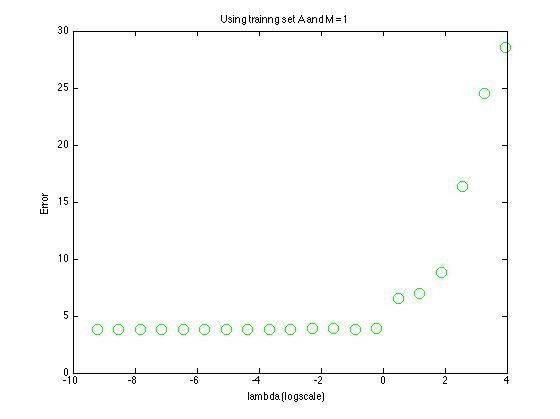
\includegraphics[width=\linewidth]{figures/p4_LAD_regressA_m=1}
\endminipage\hfill
\minipage{0.32\textwidth}
  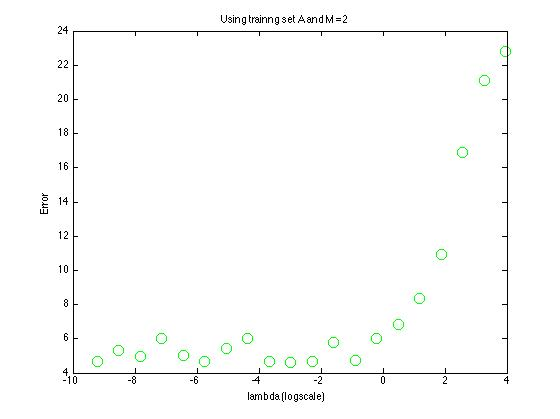
\includegraphics[width=\linewidth]{figures/p4_LAD_regressA_m=2}
\endminipage\hfill
\minipage{0.32\textwidth}                                                                                 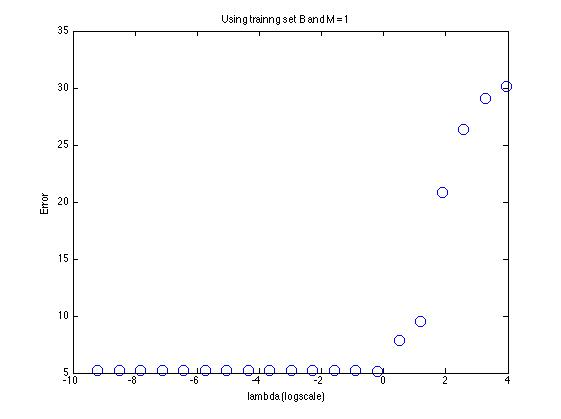
\includegraphics[width=\linewidth]{figures/p4_LAD_regressB_m=1}
\endminipage\hfill
\minipage{0.32\textwidth}
  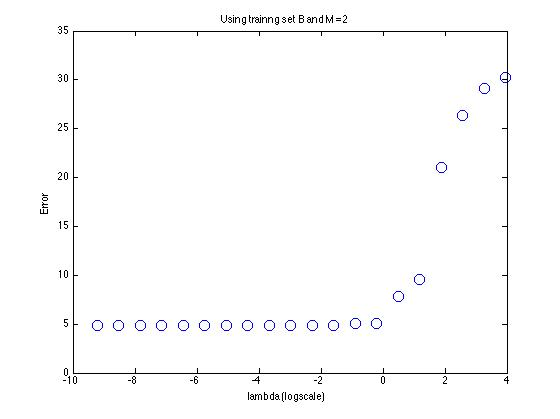
\includegraphics[width=\linewidth]{figures/p4_LAD_regressB_m=2}
\endminipage\hfill
\caption{LAD}
\end{figure}

My experiments on validation set shows that M = 1, M = 2 generates the
best results. We carried out a series of experiments with varying values
of lambda, setting M = 2 and 3. We tested for training set A and B. 

We first notice that the model generated from training set B's error
is comparable to the models generated from training set A. The minimum of
both models is around 5. We belive the reason to that is that the 
LAD model uses an absolute value based loss function that penalizes less
on outliers compare to the squared error loss function. 

Additionally, as the error is small for both models. There is no clear 
inflation point as we increase the lambda. We chose the best M and lambda
for A (M = 2, lambda = 0.01) , for B (M = 2, lambda = 0.01) using the LAD's loss function.  Then, we tested the two models on the test set, which we created from the validation set. 
%TODO: test it on the test set
The error we see on the test set is very similar to the error in the validation set. 


\subsection{Part2}

\begin{figure}[!htb]
\minipage{0.32\textwidth}
  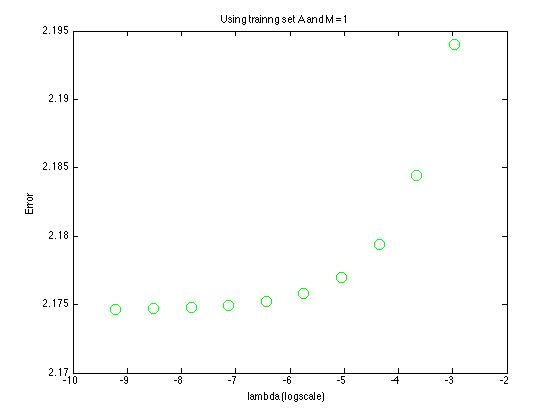
\includegraphics[width=\linewidth]{figures/p4_LASSO_regressA_m=1}
\endminipage\hfill
\minipage{0.32\textwidth}
  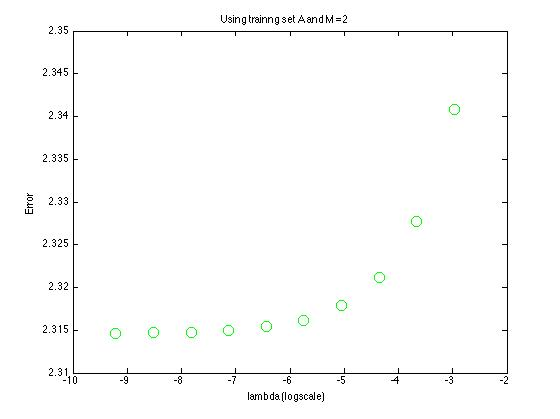
\includegraphics[width=\linewidth]{figures/p4_LASSO_regressA_m=2}
\endminipage\hfill
\minipage{0.32\textwidth}                                                                                 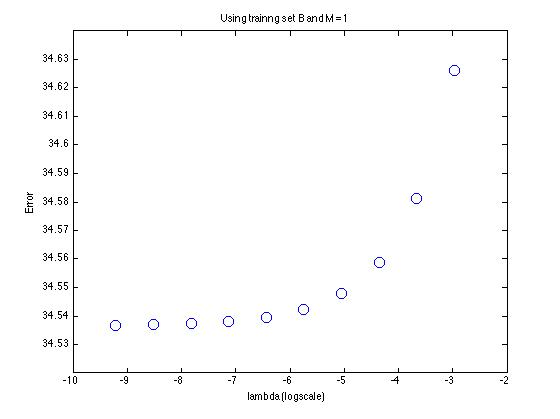
\includegraphics[width=\linewidth]{figures/p4_LASSO_regressB_m=1}
\endminipage\hfill
\minipage{0.32\textwidth}
  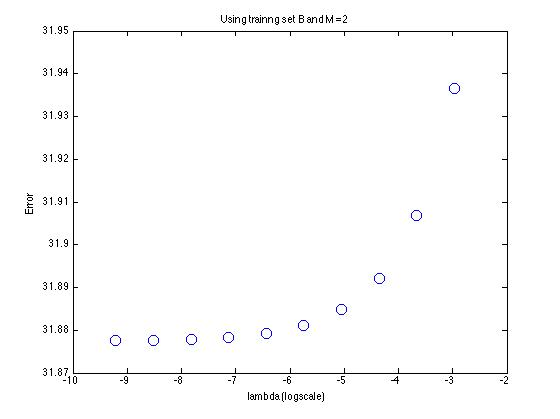
\includegraphics[width=\linewidth]{figures/p4_LASSO_regressB_m=2}
\endminipage\hfill
\caption{LASSO}
\end{figure}


The error rate for LASSO increases quickly for M = 2 and M = 3.


\subsection{Part3}
We want to use the least absolute deviations
when we believe that there are outliers in your training data. As we can see, model trained using LAD
has much lower error rate compare to LASSO and SSE on training set B. When we are confident about the quality of the data (very few or no outliers), then using a squared error loss function would be more accurate in training the model. LASSO uses L1 norm for regularization to make the weight factors more sparse. 
%TODO: add more content to the explanation
I tried using larger Ms and noticed more weights are driven to 0 when using Lasso. 
